\section{File Descriptors}
Il file descriptor è un'astrazione (integer, inizio buffer) dell'os, e quindi multi linguaggio, per permettere l'accesso ai file.

Ogni processo ha la \textbf{file descriptor table} di record indiretti delle informazioni (file descriptor) sui file aperti dal processo stesso.
I record sono indiretti perchè puntano ai record della \textbf{tabella di sistema}. La tabella di sistema contiene file descriptor dei file attualmente aperti.

Un processo/shell figlia eredità una copia della f.d. table, successivamente modificabile. Padre e figlio si devono sincronizzate sull'accesso ai file. Ciò permette un modo di comunicazione tra i processi.

Rindizionamenti:
\begin{itemize}
	\item \textbf{Processi figlio}: Padre può cambiare le associazioni fd/stream passate al figlio.
	\item \textbf{Auto-ridirezionamento}: fd viene associato a stream diverso.
\end{itemize}

\begin{center}
	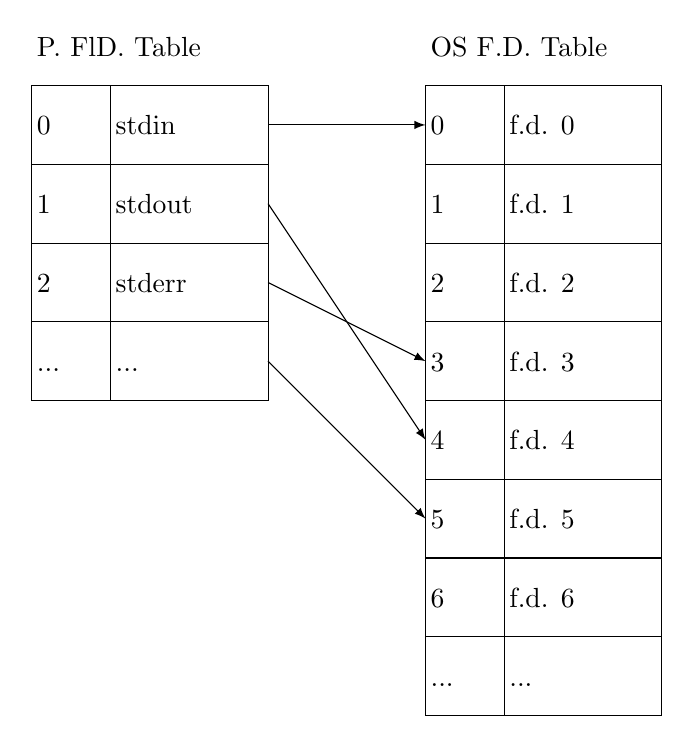
\begin{tikzpicture}
		\draw[draw=black, thin, solid] (-5.00,4.00) rectangle (-2.00,0.00);
		\draw[draw=black, thin, solid] (-4.00,4.00) -- (-4.00,0.00);
		\draw[draw=black, thin, solid] (-5.00,3.00) -- (-2.00,3.00);
		\draw[draw=black, thin, solid] (-5.00,2.00) -- (-2.00,2.00);
		\draw[draw=black, thin, solid] (-5.00,1.00) -- (-2.00,1.00);
		\node[black, anchor=south west] at (-5.06,3.25) {0};
		\node[black, anchor=south west] at (-5.06,2.25) {1};
		\node[black, anchor=south west] at (-5.06,1.25) {2};
		\node[black, anchor=south west] at (-5.06,0.25) {...};
		\node[black, anchor=south west] at (-4.06,3.25) {stdin};
		\node[black, anchor=south west] at (-4.06,2.25) {stdout};
		\node[black, anchor=south west] at (-4.06,1.25) {stderr};
		\node[black, anchor=south west] at (-4.06,0.25) {...};
		\node[black, anchor=south west] at (-5.06,4.25) {P. FlD. Table};
		\draw[draw=black, thin, solid] (0.00,4.00) rectangle (3.00,-4.00);
		\draw[draw=black, thin, solid] (1.00,4.00) -- (1.00,-4.00);
		\draw[draw=black, thin, solid] (0.00,3.00) -- (3.00,3.00);
		\draw[draw=black, thin, solid] (0.00,2.00) -- (3.00,2.00);
		\draw[draw=black, thin, solid] (0.00,1.00) -- (3.00,1.00);
		\draw[draw=black, thin, solid] (0.00,0.00) -- (3.00,0.00);
		\draw[draw=black, thin, solid] (0.00,-1.00) -- (3.00,-1.00);
		\draw[draw=black, thin, solid] (0.00,-2.00) -- (3.00,-2.00);
		\draw[draw=black, thin, solid] (0.00,-3.00) -- (3.00,-3.00);
		\node[black, anchor=south west] at (-0.06,4.25) {OS F.D. Table};
		\node[black, anchor=south west] at (-0.06,3.25) {0};
		\node[black, anchor=south west] at (-0.06,2.25) {1};
		\node[black, anchor=south west] at (-0.06,1.25) {2};
		\node[black, anchor=south west] at (-0.06,0.25) {3};
		\node[black, anchor=south west] at (-0.06,-0.75) {4};
		\node[black, anchor=south west] at (-0.06,-1.75) {5};
		\node[black, anchor=south west] at (-0.06,-2.75) {6};
		\node[black, anchor=south west] at (-0.06,-3.75) {...};
		\node[black, anchor=south west] at (0.94,-3.75) {...};
		\node[black, anchor=south west] at (0.94,2.25) {f.d. 1};
		\node[black, anchor=south west] at (0.94,3.25) {f.d. 0};
		\node[black, anchor=south west] at (0.94,1.25) {f.d. 2};
		\node[black, anchor=south west] at (0.94,0.25) {f.d. 3};
		\node[black, anchor=south west] at (0.94,-0.75) {f.d. 4};
		\node[black, anchor=south west] at (0.94,-1.75) {f.d. 5};
		\node[black, anchor=south west] at (0.94,-2.75) {f.d. 6};
		\draw[draw=black, -latex, thin, solid] (-2.00,0.50) -- (0.00,-1.50);
		\draw[draw=black, -latex, thin, solid] (-2.00,1.50) -- (0.00,0.50);
		\draw[draw=black, -latex, thin, solid] (-2.00,2.50) -- (0.00,-0.50);
		\draw[draw=black, -latex, thin, solid] (-2.00,3.50) -- (0.00,3.50);
	\end{tikzpicture}
\end{center}

In POSIX per ogni processo i file descriptor standard sono: stdin=0, stdout=1, stderr=2.

Ricoda che stdin è lo stream input da tastiera e stdout e stderr sono gli stream a video dell'output e dei messaggi d'errore.

Nota: Processi diversi possono avere file descriptor diversi, ma constesso valore, e che referenziano file diversi.

In C per scrivere si usa <fprintf(stdout/stderr, "..." [, parametri])> e per leggere si usa <fgets(buffer, size, stdin)>, per il fine file usare <feof(stdin)>.